\section*{Exercise T-3.2}
\subsection*{Problem}
We consider a two-category $(\omega_1 , \omega_2 )$ two-dimensional $(x_1, x_2 )$ classification problem. Assume that the given 4 data points for each class
\begin{align}
\omega_1 :& \quad \{(3,8),(2,6),(3,4),(4,6)\}\nonumber\\ 
\omega_2 :& \quad \{(3,0),(3,-4),(1,-2),(5,-2)\}\nonumber\\ \nonumber
\end{align}
are normally distributed and that the priors of both classes are equal.\\

Compute the decision boundary and specify it as a function of $x_1$ , i.e. $x_2 = f (x_1 )$. Illustrate the boundary together with the two point clouds in an appropriate diagram.\\

It is not allowed to use a computer (Octave, Matlab, ...) to solve this task.

\subsection*{Solution}

We could not find a mathematically calculated formula for a function $x_2=g(x_1$).\\
As the priors of the classes are equal and therefore have the same prior propability ($0.5$), we assumed that the decision boundary would be a horizontal line at $x_2=2$ as this would be the mean between the means of the two pointclouds $\omega_1$ and $\omega_2$ which both are \textit{symmetric} as shown in figure \ref{img:pointCloud}. Intuitively, for every $x_1$, the equation $p(x|\omega_1)\cdot p(\omega_1) = p(x|\omega_2)\cdot p(\omega_2)$ would be fulfilled on $x_2=2$
\begin{figure}[b]
	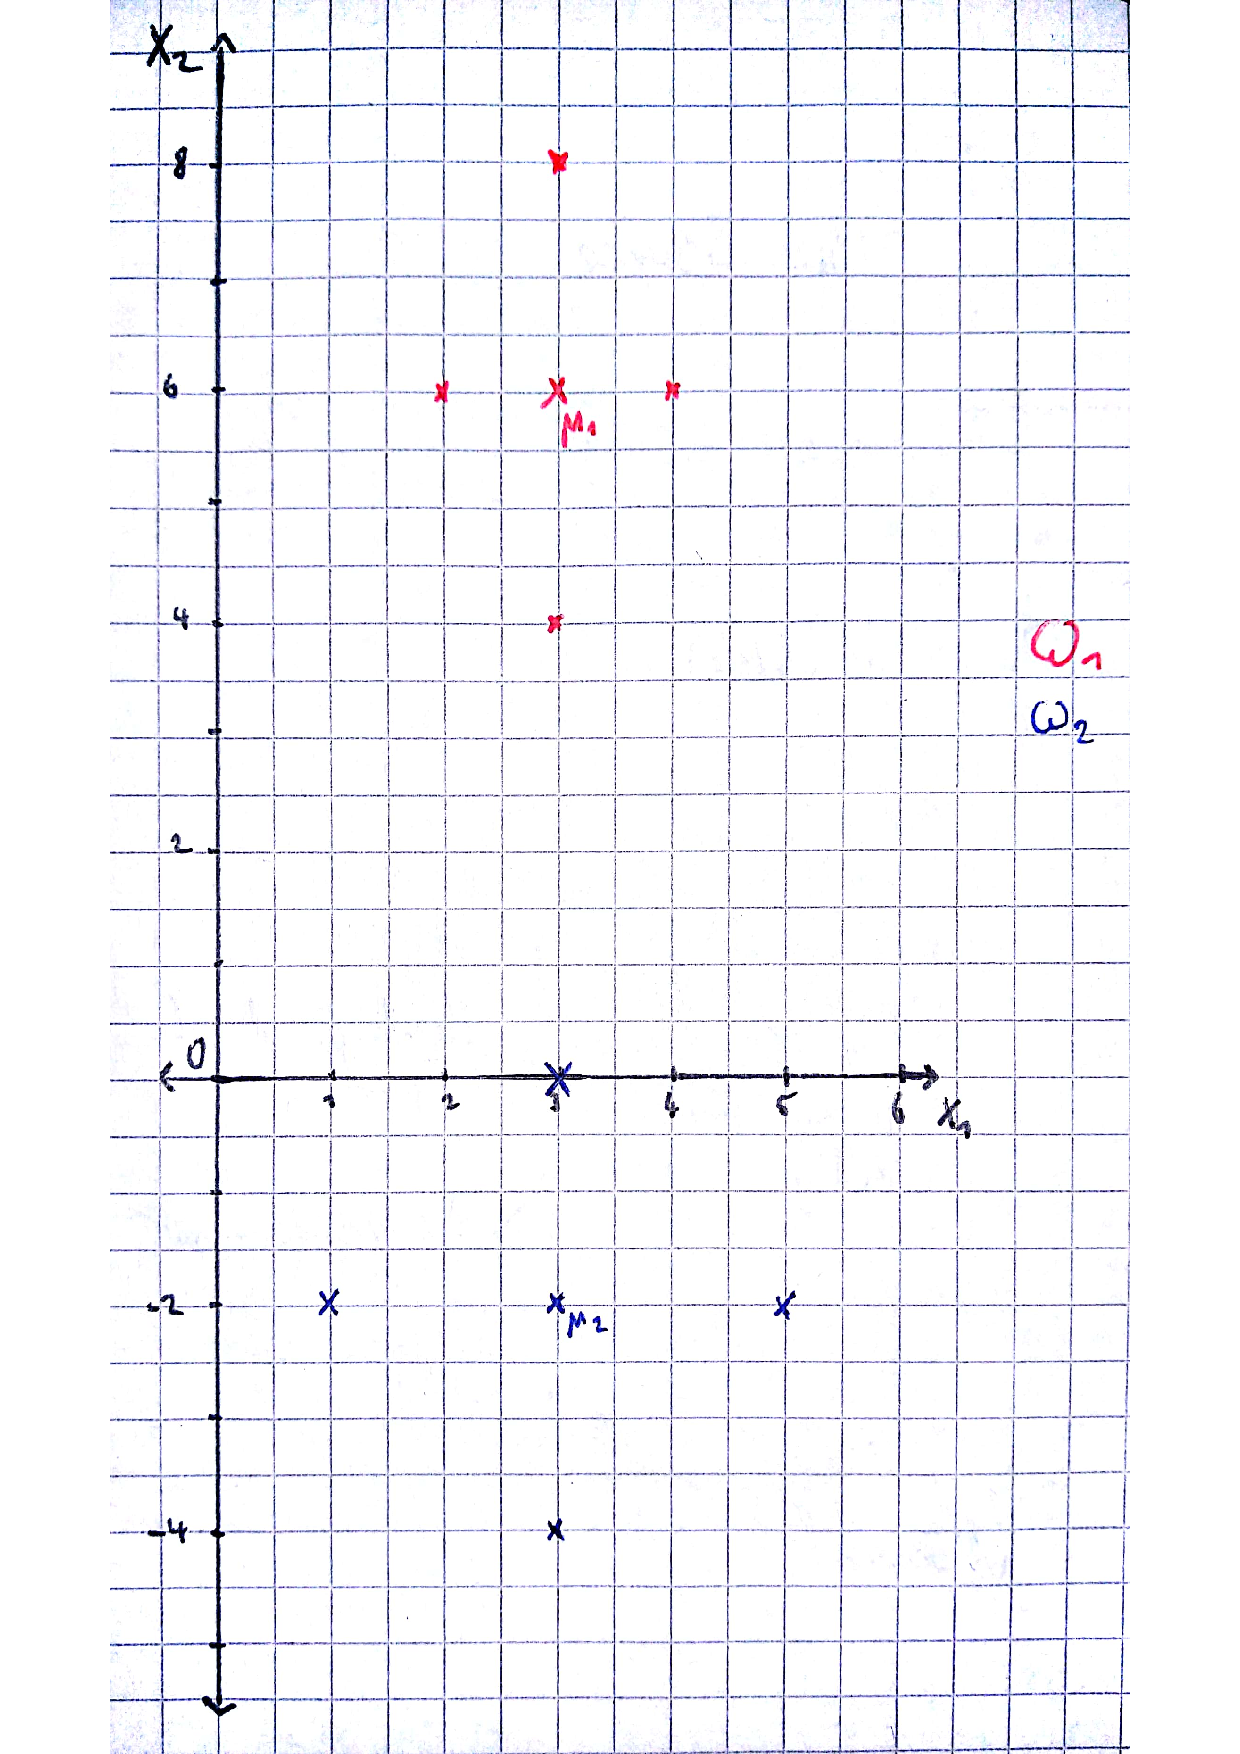
\includegraphics[width=1\linewidth]{pointCloud2}
	\caption{text}
	\label{img:pointCloud}
\end{figure}
